\documentclass[10pt,final,conference]{IEEEtran}
%\documentclass[10pt,final,conference]{article}

\usepackage{amsmath,amsfonts,amssymb,amscd,amsthm,xspace}
\usepackage{algorithm}
\usepackage{algorithmic}
\usepackage{graphicx}
\usepackage{caption}
\usepackage{subcaption}
\usepackage[square, numbers, comma, sort&compress]{natbib}
\usepackage{fancyhdr}
\usepackage{listings}
\usepackage[colorlinks,linkcolor={black},citecolor={blue}, urlcolor=black]{hyperref}

\begin{document}

\title{Final Project: Asteroid Planning}
\author{Robot Intelligence: Planning 4649/7649 \\
Group 2: Kyle Volle, Luke Tornquist, Steffan Slater, Xinyan Yan}
\maketitle

%\tableofcontents{}

\newpage

\nocite{*}

\begin{abstract}
In this paper, planning and machine learning concepts are applied to the design of an autonomous agent to play an "asteroids" type computer game. The game presents unique challenges in limited movement range, spawning of more and smaller asteroids after a bullet impact, and elastic asteroid-asteroid interactions. Two components of the game are investigated - selecting a direction in which to move the craft and selecting a direction in which to fire bullets in an attempt to destroy asteroids and increase the score. A velocity obstacle approach is used to determine safe directions for the craft to travel, and one of those safe headings is selected in one of several manners. The results of many runs with different direction selecting and firing combinations are presented. (velocity obstacle approach analysis). The previewer which picks a heading from the plausible heading pool is probabilistic optimal in terms of the sum of discounted rewards $n$ steps into the future.  

\end{abstract}

\section{Member Responsibilities}
For this project, Kyle was in charge of writing the introduction and putting together the results and plotting the data, both in the paper as well as in the presentation.  Luke developed the Asteroids game, and created the remote interface for the planner to utilize.  Luke also worked on the decision tree algorithm that is utilized in calculating when the ship should fire and when it should not.  He also typed up the relevant sections in the paper and put together the video for the presentation.  Steffan wrote all of the Navigation planning algorithm, which does almost all of the motion planning for the ship.  He also did a significant amount of research regarding the planning algorithms that have been historically associated with the asteroids problem.  He also typed up all his relevant parts in the paper, and presentation.  Xinyan worked on creating the motion planning machine learning, that was to be used for helping determine which "safe" heading to choose when multiple are present.  Due to time constraints and other unforseen circumstances, the motion planning machine learning was not completed, but instead Xinyan completed the Preview planning algorithm.  Xinyan also worked on typing up his relevant parts in the paper and presentation.

\section{Introduction}
The "asteroids" genre of games poses several interesting planning problems. In this game, the player controls a spaceship in an environment that is filled with fast moving obstacles called asteroids. Collision with an asteroid causes the player to lose a life. Points are scored by shooting the asteroids and breaking them into two smaller, faster obstacles. Asteroids progress from large to medium to small. If a small asteroid is hit, it is removed from the game. As the game goes on more and more obstacles are spawned. The goal for the player then is to stay alive as long as possible to keep shooting asteroids.

This game is interesting for several reasons. For starters there is no final goal, but rather the planner seeks to stay alive for as long as possible. This differentiates this problem from more traditional motion planning problems. Additionally, in this game there are no static states. Conservation of momentum keeps the ship moving at a constant velocity if there is no player input. Combined with the dynamic nature of the obstacles, the game state can change rapidly requiring frequent replanning.

The planner utilizes several processes in order to maximize the potential future score. An array of safe trajectories is first calculated and from this list another process selects one of these trajectories based on the anticipated rewards and costs. Finally, a third process determines the game inputs corresponding to following this trajectory and places these inputs in an executor queue to be performed as the replanning occurs. Factors for selecting a trajectory include, but are not limited to, time required to achieve that trajectory, density of asteroids along the trajectory, distance to obstacles along the trajectory and the ability to destroy asteroids along the way. The Methods section will go into greater detail about the techniques and strategies employed.

\section{Related Work}

A significant amount of literature exists for the problem of navigation with mobile obstacles. This literature tends to fall into one of two categories - local methods or global methods, based on how obstacles influence robot behavior \cite{khansari2012dynamical}. Local methods include bug algorithms and the Vector Field Histogram, while global methods include artifical potential fields and visibility graphs. Local methods tend to run rapidly but may not find feasible paths, while global methods will find a valid solution if there is one but tend to be slow. Given that our environment can be frequently changing as asteroids collide or are struck by bullets and break apart, a local method would appear to be a better choice to allow for rapid replanning; however, including some ability to look ahead is critical in an environment with moving obstacles. 

The selected approach for navigation planning is based on the concept of velocity obstacles, which takes into account all future obstacle/robot future relative positions, assuming constant velocities \cite{fiorini1998motion}. The constant velocity assumption is acceptable for our problem as the plan will be rebuilt frequently, which will account for any asteroid-asteroid or asteroid-bullet interactions. While the exact approach used will be described in detail later, the concept is to convert the space and time domain into a purely spatial representation which can be easily searched for collisions. This results in a velocity space representation of the robot and obstacles, which is then used for planning. This approach, unlike some navigation methods, generalizes well to real-world applications of robots with limited sensors and domain knowledge, and has been used for autonomous surface vessel navigation in the crowded Singapore harbor \cite{bandyophadyay2010simple}. 

\section{Methods}

\subsection{Game Development}
We decided to develop the game ourselves due to the lack of open source projects that had all the functionality that we desired.  We utilized LibGDX as the basic framework for creating the game.  LibGDX is built on Java, so we decided to use Java for the planner as well.  The game mechanic that we really wanted in our game was to have realistic physics in regard to collisions.  Most open source games out there do not have this feature, as the original Asteroids game did not have it either.  We added this functionality using the Box2D libraries that come built in to LibGDX.  This allowed us to give asteroid collisions a more realistic feel, and it also made the game a good bit more difficult.  Another very important reason that we chose to develop the game ourselves was the fact that it allowed us to get access to any data that we needed from the game.  We created all of the entities (Ship/Asteroids) as circular objects to simplify our calculations.  The textures that we used, also seemed to be that way, so it fit well.

\subsection{Game and Planner Interface}
The planner interfaces with the game using Remote Method Invocation (RMI).  This method of remote calls is supported in Java to allow interprocess communication.  This is how we transfer game data from the game to the planner, as well as transfer plan actions from the planner to the game.  The way it works is pretty basic as it functions much like a client/server model.  The Game functions as the RMI Server and registers with the local RMI Registry to expose the interface to other processes.  The Planner functions as the RMI Client and queries the RMI Registry for the exposed interface.  This returns as shared object that allows the planner to call any exposed methods remotely.

\begin{figure}[ht]
\centering
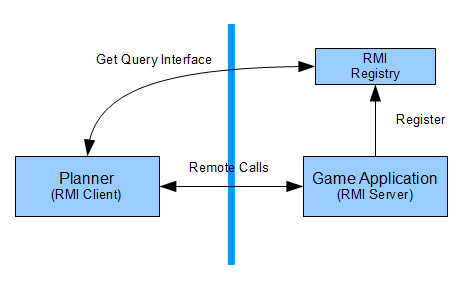
\includegraphics[width=3in]{./RMI.png}
\caption{RMI Basics}
\label{fig_rmi}
\end{figure}

\subsection{Navigation Planning}

The navigation planning approach is based upon the velocity obstacle method described in \cite{fiorini1998motion}. The motion of the robot and a single obstacle is transformed into relative motion of the robot and a stationary obstacle at the same current position. The asteroid is then expanded by the radius of the robot plus a safety factor. This safety factor prevents this method from being complete, as it can cause the planner to miss potential feasible passages, but compensates for inaccuracies in the turning maneuvers and the slight lag of the planner behind the actual game execution. This expansion of the asteroid collapses the spacecraft to a point, moving the problem into the more tractable configuration space. 

After expanding the asteroid, the exclusion cone of the obstacle is computed. This cone consists of two rays from the current robot position through the tangency points of the obstacle. Since the velocity obstacle approach transforms a moving obstacle to a stationary one, any robot velocity relative to the obstacle which falls into the exclusion cone will at some point result in a collision. The current relative velocity of the robot to the obstacle is then placed in the space, and may or may not be within the exclusion cone of the obstacle. It is then necessary to compute the range of possible relative velocities after some amount of time.

The computation of the possible relative velocities is accomplished by computing the potential change in velocity in each direction based on the robot's current attitude. In Asteroids this presents an interesting problem, as the space of potential velocity changes is not a simple shape. While a two-degree-of-freedom actuated effector such as the print head on a 3D printer has a rectangular velocity change space (as the two directions are independent), and a vehicle which can apply a thrust linearly in any direction has a circular velocity change space, the craft in Asteroids can only accelerate forward and has a finite turn speed. This means that for a given amount of time, the craft can accumulate more change in velocity in a forward direction than in any other direction, as it must first turn before accelerating in that direction. This results in a heart-shaped velocity change space given by the equation:

\begin{equation*}
\Delta v(\theta) = a \left( \Delta t - \frac{\theta}{\omega} \right)
\end{equation*}

where $a$ is the acceleration of the craft and $\omega$ is the angular velocity while turning. This velocity change space is then rotated by the craft attitude and translated by the relative velocity to obtain the set of reachable relative velocities within the time step. The time step used is the time required to perform a 180-degree turn and accelerate to 25\% of the ship maximum velocity or the shortest time to impact, whichever is smaller. 

The set of reachable relative velocities is then intersected with the exclusion cone to find which directions (headings) are safe for the craft to move along. This is done by calculating the angle from the current position to each point on the reachable velocity curve and searching for all points where that angle is equal to the angle of the edges of the exclusion cone, as those tangent lines are lines of constant angle (radial lines in polar coordinates). Which side of the intersection heading is safe is determined by picking a point on either side and taking the sum of the angles between the tangent lines and a line though the current position and that point. If the sum is equal to the angle between the two tangent lines, it is between the two and therefore in the exclusion zone. If that sum is greater than angle between the two tangents, it is outside the exclusion zone. This strategy will give the safe and unsafe heading ranges for the craft based on a single obstacle. The results for all obstacles can then be superimposed to get the overall safe and unsafe ranges. An example of a reachable velocity region with an exclusion cone is shown in Figure \ref{fig:reachable_veloc}, with the relative velocity in blue, the axis of the craft in dashed black, the reachable velocities in solid black, and the boundaries of the exclusion cone in red.

\begin{figure}[ht]
\centering
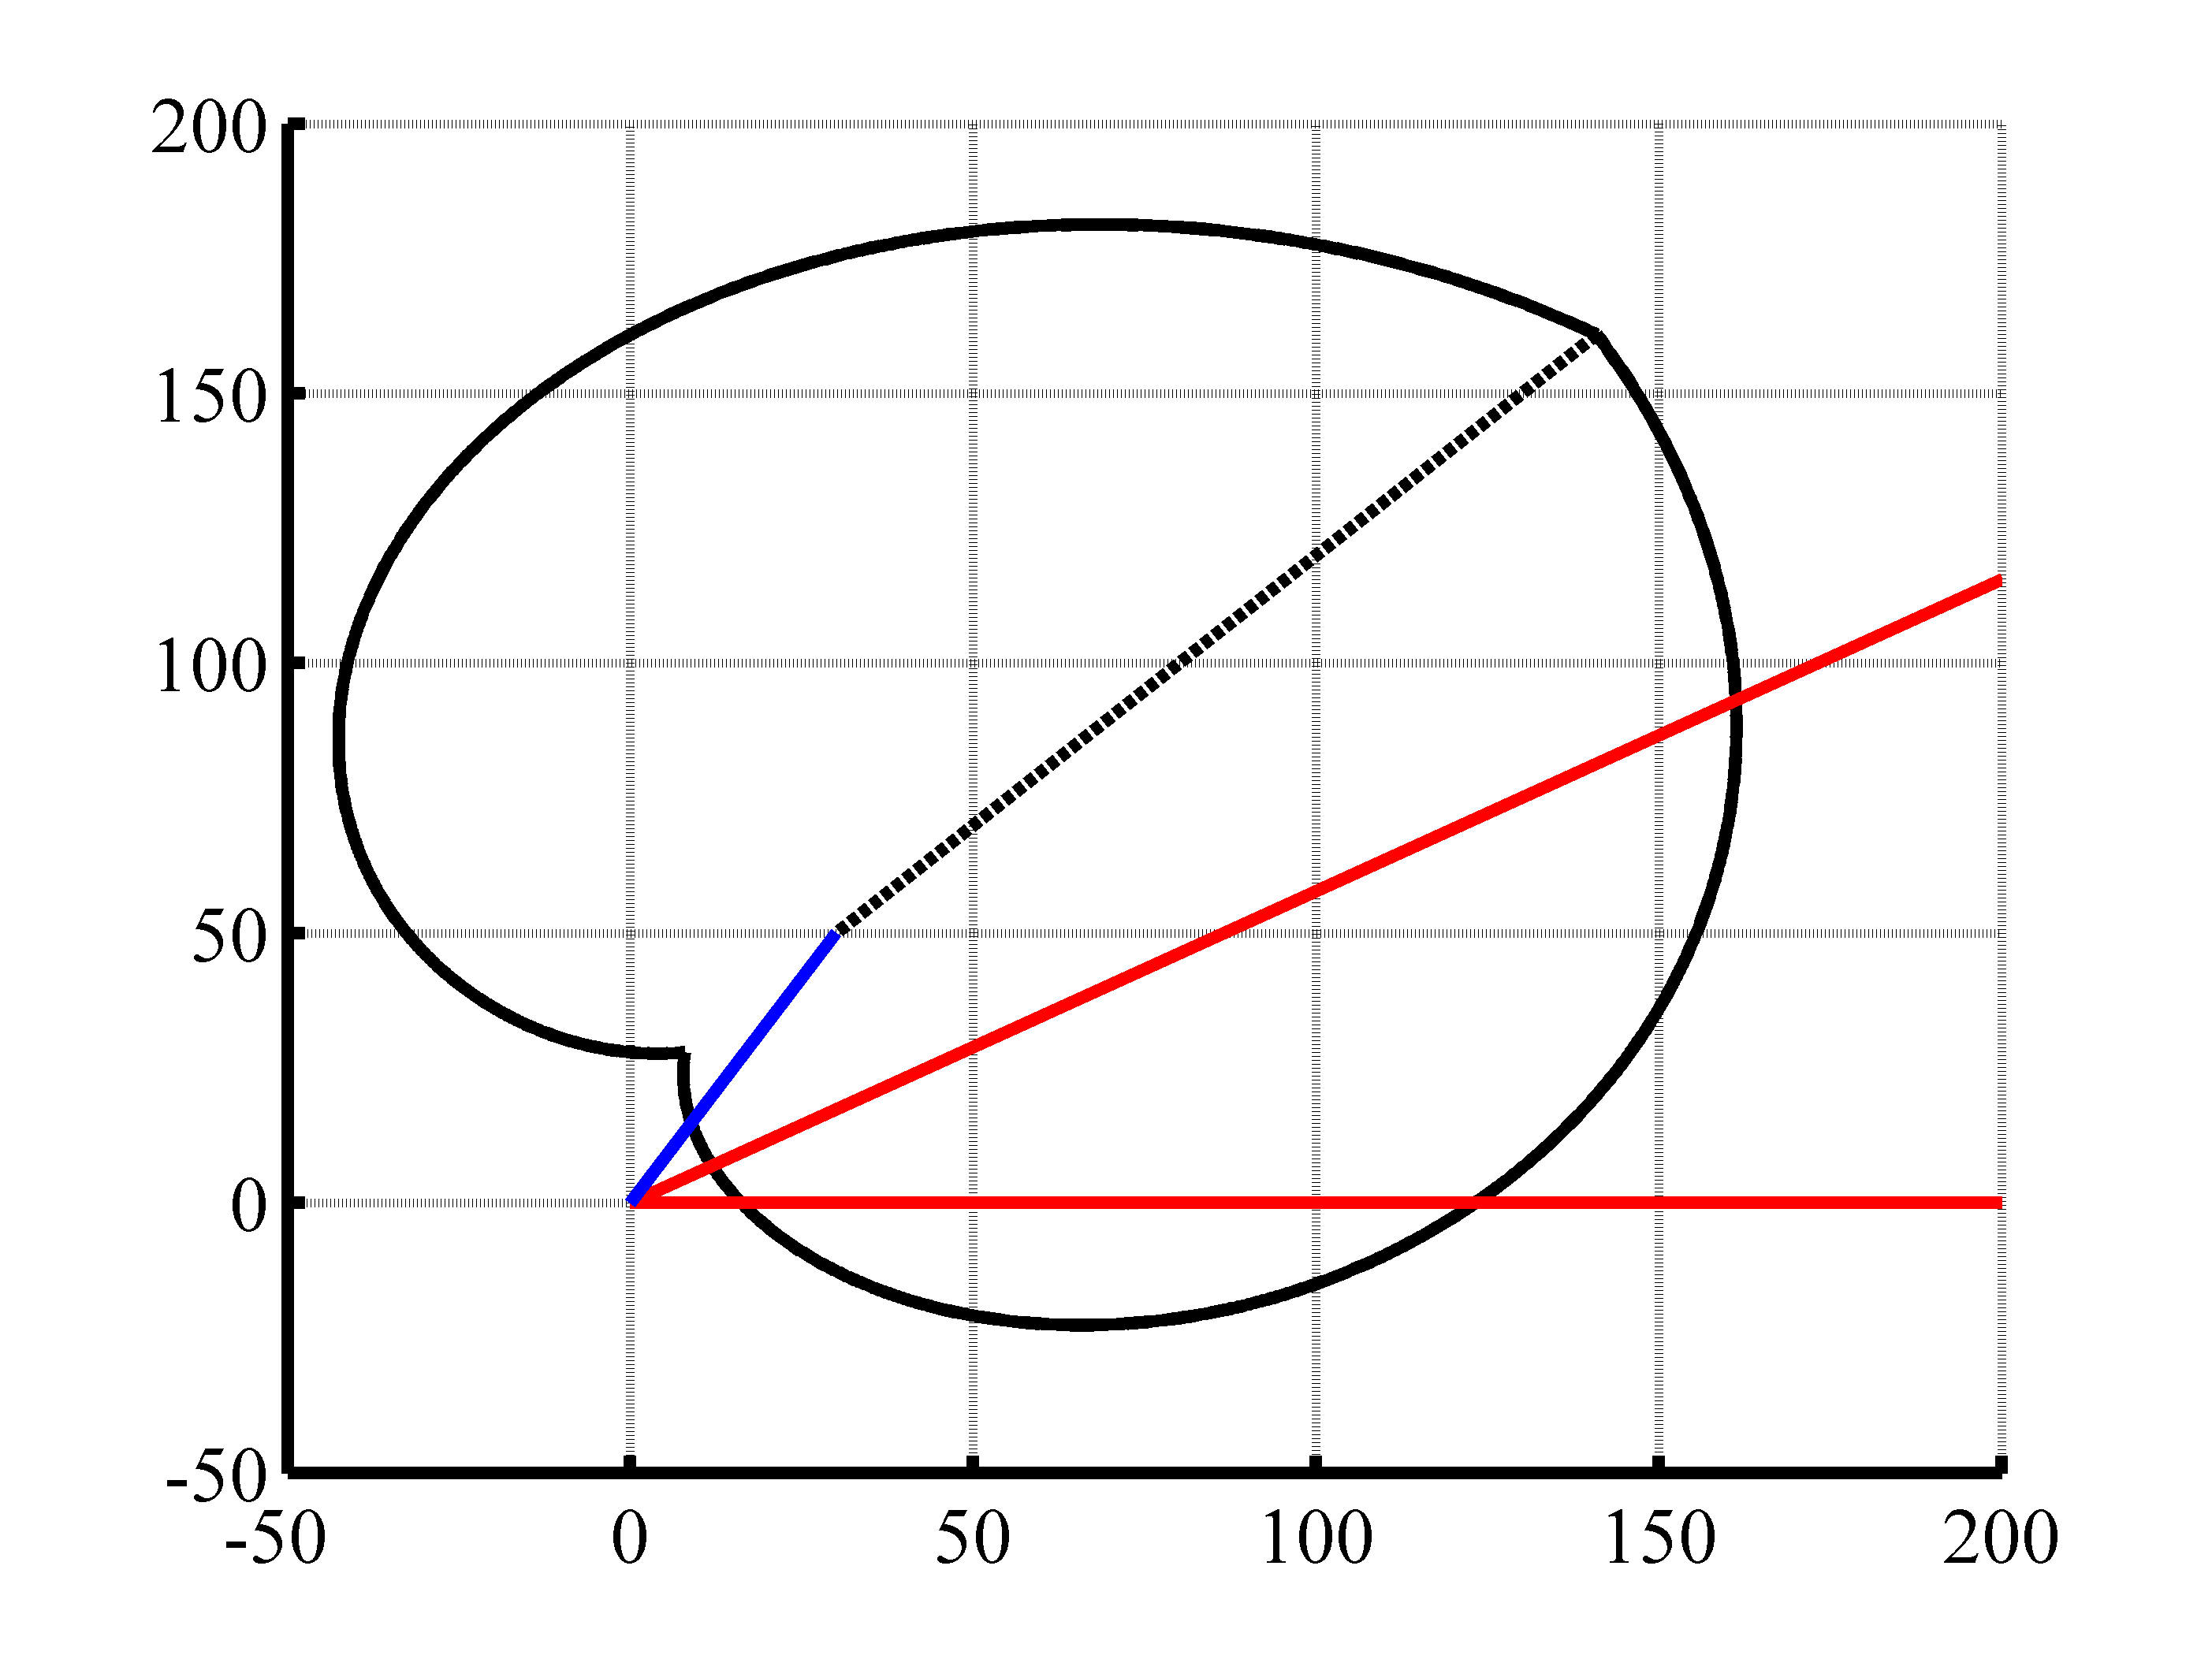
\includegraphics[width=3in]{./deltav_curve_rotated_translated_obstacle_color.png}
\caption{Reachable Velocities with Exclusion Cone}
\label{fig:reachable_veloc}
\end{figure}

To ensure that not all headings are excluded, only asteroids within some distance of the craft are considered. This distance can be modified by the planner, for example by reducing the search radius to open up more safe headings. From the set of safe headings, one heading is selected as the target and a rotation and acceleration maneuver to that heading is computed. The selection of the heading is the true job of the navigation planner. Most of the extant literature focuses on using the velocity obstacle approach to calculate a path to a goal point, but Asteroids does not have a goal point. The selection of the target heading must therefore be chosen in a different manner. One method that was considered, for example, was selecting the safe heading closest to the current direction, thereby minimizing the amount of turning that was to be carried out.

\subsection{Decision Trees}
Decision trees were used to predict whether we should or should not shoot at each particular asteroid.  We used decision trees as they allow us to classify particular situations based on a set of input variables, and learn from success and failure to learn over time.  This should allow the ship to get more adapt at figuring out when it is good to fire and when it is not.  The output of the tree is basically a classification for that particular set of variables in the tree, which correlates to the path from the leaf node to the root of the tree.  That classification maps to either true or false in our case, as we are trying to decide whether we should fire or not.

\begin{figure}
\centering
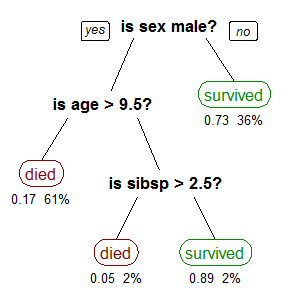
\includegraphics[width=3.0in]{./CART_tree_titanic_survivors.png}
\caption{Decision Tree - Example\cite{titanic}}
\label{fig_decision_tree_example}
\end{figure}

Figure [\ref{fig_decision_tree_example}] is an example decision tree that was used as a basis for the decision tree creation for the Asteroid Planner\cite{wikiDecisionTreeLearning}.  It was used as an example because we needed to persist a similar kind of data, which is basically a numeric value which corresponds to the success rate of firing mapping to a successful outcome.  This numeric value is then used to predict whether we should fire or not.  Similar metrics are used in Figure [\ref{fig_decision_tree_example}] except the outcomes are died or survived.

\begin{figure}
\centering
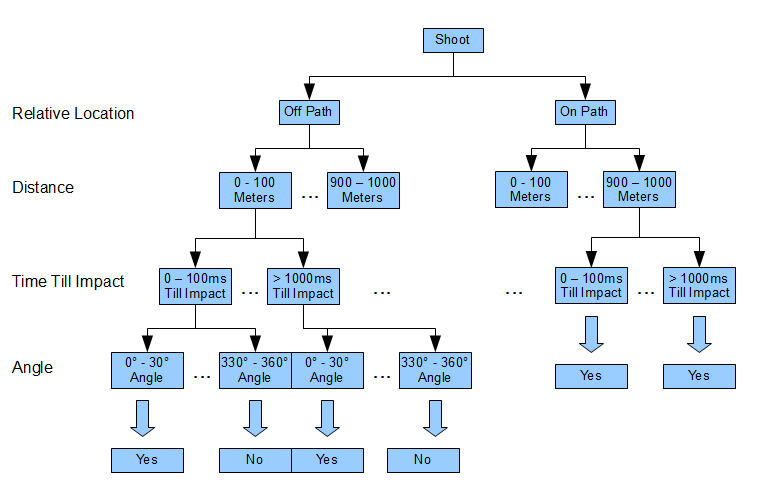
\includegraphics[width=3.0in]{./DecisionTree.png}
\caption{Decision Tree - Asteroids Planner}
\label{fig_decision_tree_asteroids}
\end{figure}

Figure [\ref{fig_decision_tree_asteroids}] is the layout of our decision tree that we utilized for fire planning in our system.  We used a few metrics that would help classify every asteroid each time we analyzed it.  The first metric was relative path, and it was simply a true or false value that was true if the asteroid could cross our line of sight as we avoided any obstacles, and false otherwise.  The next metric is the distance that the asteroid is from the ship, which can obviously be a very helpful metric.  Another metric we decided to use was the time till impact.  This takes into account not only the distance of the asteroid, but also the velocity of that asteroid.  Finally, the last metric we decided to use was the angle that the asteroid was from our current ship heading.  Since some of these metrics were numeric, rather than boolean, we decided to segment each of the metrics into ranges, and use those as a more granular way to classify the asteroids.  In Figure [\ref{fig_decision_tree_asteroids}] you can see the ellipsis' between the nodes that have ranges, because they are there to represent the numerous nodes that would exist between the two nodes.

At each leaf, we keep a few pieces of vital information that we use to determine the usefulness of the data as well as the predictability.  

\subsection{Preview Planning}
Navigation planning provides a range of safe headings to take. A previewer is used to pick a heading from the pool at each time when decision needs to be made in our case. MDP, POMDP and LQR had been considered to solve this problem. If state is defined as the velocity, position and angle of the ship and asteroids in MDP, then because of the things that are hard to predict, like newly periodically created asteriods, collisions of asteroids, dynamics of the ship, and the state transition probability are really hard to compute. What's more, the dimension of the state space is high, 9 asteroids plus 1 ship lead to 33 dimension. With discretization, we might end up with $10_33$ states. With regard to POMDP, sensing error is taken into account, which does not exist in our settings, because state is known exactly through querying the game server. Finding a shorter state description might be plausible, but the transition table still needs to be learnt first, which would still be very huge. LQR is not applicable either, because the dynamics of the ship might not be linear, and good performance criterion can not be represented in a quadratic form.

So, we ended up with using a naive method--previewing just several steps into the future, as the state is only predicable within a certain amount of time. Heading samples are the possible actions to take. And high reward can be achieved if the resulted state looks good(high safe heading percentage, far from the nearest asteroid), and the turn angle is small. 


\begin{equation} \nonumber
\begin{split}
\text{States\ \ \ \ }\ &\sum = \{s_1,..., s_n\}  \\
\text{Actions\ \ \ \ }\; &A = \{a_1,..., a_n\} \\
\text{Rewards\ \ \ \ }\; &R = \{r(s_i, a_j)\} \\
\end{split}
\end{equation}

\textit{States} are angle, position and velocity of the ship and asteroids. \textit{Actions} represent different headings. \textit{Rewards} are the rewards we will get if we take actions in given states.
The optimal action $\hat{a}$ to take in state $s_i$ would be:
\begin{equation} \nonumber
\begin{split}
\hat{a} =& \arg\max_{a}  ( r(s_i, a) + \gamma r(s_j, a_m) + \gamma^2 r(s_k, a_n) + ... \\
 &+ \gamma^{n-1} r(s_l, a_o)  ) 
\end{split}
\end{equation}
In the equation, $s_i \rightarrow s_j \rightarrow s_k \rightarrow ... \rightarrow  s_l$ is a sequence of states.
Because the dynamics of asteroids and ships are deterministic, and we know the state exactly by reading game data, we don't have execution error or sensing error, which makes preview planning very simple. Although we do have uncertainty about where new asteroids will be created at what velocity, we neglect it because of its high complexity and not influential in a short time. To solve this problem, we build a tree, in which nodes denote states and edges denote actions associated with discounted rewards. The edges are associated with rewards which indicate the immediate rewards by taking the actions in those states. Instead of enumerating the sum of discounted rewards of all the paths, we trace back the tree to find a maximal path. Then we choose the first action in the path to take. 

\section{Experiments}

The way we ran the experiments was by allowing the planner to restart the game, it allowed the planner to automatically play numerous games in a row.  We also allowed a variable to be modified that would gate what portions of the planner were executed.  So you could run the planner with any combination of Navigation, Decision Tree, Constant Fire, or Preview planning.  Each flag would gate a different piece of the planner so that we could see how each piece would behave alone or together with other pieces.  Generally speaking, we used the score as the main evaluation for our algorithms as that is the main purpose of the game.  We also tracked the game time as well, as there could be a component added to the game that would allow accruing of points over time that may influence how well an algorithm performs.

For the Decision Tree piece, the Decision Tree object is serialized out into a file so that even if the planner is closed, it will load up the decision tree from the last avaiable state.  We also added an element into the planner so that it dumps the current state of the Decision Tree along with the Score and Game Time out to a CSV file after each game.  So we can have a running comparison of the Decision Tree state as it changes, as well as the game time and score as that tree changes.

For the Preview piece, we tweaked several parameters--1) running frequency of planner(100ms, 300ms, 1000ms), (2) number of future steps taken into account(1, 2), and (3) penalty for turn angles(0.05, 0.1). Because the ship needs relative quick reaction, and the number of nodes of the tree increase exponentially with the horizon which takes much more time to compute the best path, we only tested horizon 1 and 2. What's more, and we compared the performance of previewer and nearest safe methods for dodging without firing.

Overall, we did a variety of experiments with different flags on and off.  Each had their respective positives and negatives, but the details of those will be covered in the Analysis section.

\section{Analysis}

The velocity obstacle method as presented in \cite{fiorini1998motion} is a complete algorithm for constant velocity obstacles without interactions. The modification to the velocity obstacle method used in this project sacrifices completeness for computational simplicity. The safety factor applied to the radius of the spacecraft inherently prevents the algorithm from being complete, as it can close off small passages through which the craft would fit with small clearances. This should (depending on the magnitude of the safety factor) have a small effect as most clearances will still be sufficiently large and the compensation for planner lag and small position and attitude errors is more important. A much larger impact on the completeness of the algorithm is the limiting the selection of the reachable velocities to the boundary of the reachable region, rather than the entire area. Strictly speaking, any velocity within the region is reachable, but limiting it only to the boundary immensely simplifies the necessary computations. This simplification, which always attains the maximum velocity change in the chosen direction, was also undertaken when planning for an autonomous surface craft avoiding obstacles in Singapore harbor \citep{bandyophadyay2010simple}. Limiting the radius of consideration for obstacle avoidance (obstacles outside that distance are ignored) also decreases completeness, as obstacles outside that range could be on impact paths. Rapid replanning mitigates this concern.

The optimality of the velocity obstacle method depends on the metric used to define optimality. If optimality is defined as the shortest path to a goal, selecting the safe heading which moves closest to the goal point is locally optimal, not globally, as information outside the search radius is not available. This method can also be optimal for a goal of maintaining a specific direction or in a Voronoi sense, maximizing distance from collision velocities. Again, this is local optimality due to the search radius cutoff. This velocity obstacle calculation method is reasonably efficient - while it requires some significant math including nonlinear equation zero-finding and must run for each asteroid, the limitation of the computation to the reachable velocity boundary reduces the necessary work immensely. Using the full region requires calculating the intersection of two arbitrary areas, which is nontrivial. Ultimately, with regard to efficiency, the main concern is that the planner can keep up with the speed of the game, which it does admirably. Additionally, some of the execution time impact on performance is mitigated by shifting the planned sytem time for each action by the time required to generate the plan, which helps maintain the relative spacing of actions. Otherwise late execution of the actions early in the plan due to the planning execution time can decrease the time between actions undesirably.

The previewer that decides the best heading to pick from the plausible heading pool is probabilistically optimal. It is probabilistic because at decision time, it just does several samples from the pool instead of considering all the safe headings. It is optimal in terms of the sum of discounted rewards $n$ steps into the future, assuming state transition function we used is correct. It is probabilistically complete in terms of finding a way to survive. The planning efficiency depends on how far the future is previewed and the number of heading samples. The number of nodes in tree to trace back is $A^{H+1}-1$, and through the tracing back method, $A^H-1$ operations of finding the maximal value from $A$ numbers need to be performed.

As indicated in the experiment part, different parameters are tested. Because motion and firing are tackled seperately, which might be a large flaw in our approach, only dodging without firing cases are tested here. We ran the game 50 times for each case.


\begin{table}[!h]
\centering \small
\begin{tabular}{l|c}
  \hline
  Method &  Mean survival time(s)\\
  \hline \hline
  Nearest safe & 40.108 \\
  Previewer & 43.909 \\
  \hline
\end{tabular}
\caption{Mean survival time by using differerent heading selectors}
\label{differentmethod}
\end{table}


\begin{table}[!h]
\centering \small
\begin{tabular}{l|c}
  \hline
  Planning period(ms) &  Mean survival time(s)\\
  \hline \hline
  100 & 41.070 \\
  300 & 43.299\\
  1000 & 43.909\\
  \hline
\end{tabular}
\caption{Mean survival time by using previewer with different planning frequency}
\label{freq}
\end{table}

\begin{table}[!h]
\centering \small
\begin{tabular}{l|c}
  \hline
  Horizon &  Mean survival time(s)\\
  \hline \hline
  1 & 43.909 \\
  2 & 42.401\\
  \hline
\end{tabular}
\caption{Mean survival time by using different horizions}
\label{horizon}
\end{table}

From the above tables, we can see that previewer outperforms nearest safe by 9.5\%. And with different running frequency, it almost remains the same performance. Looking 2 steps into the future does not perform as well as looking 1 step. This maybe the case that collistions of asteriods are not taken into account and ship position propagations are not calculated exactly. The execution for an action is near 2s, during which period, the world changes a lot. 

\section{Discussion}

One of the biggest problems we had was the fact that we had to develop the game from the ground up, which sounded relatively easy from the beginning, but became more and more difficult as time went on.  It was definitely worth it for the customizability, but the scope of work grew over time.  And one of the main reasons for that is that generally speaking, games are not made to handle the insanely fast input of a computerized planner, and thus it caused numerous issues within our game.  Every few runs the game gets in a bad state and crashes, so you have to manually restart the game and planner again.  It makes running the experiments a pretty tedious process and should definitely be a consideration next time.

Another important lesson that we learned was that both the toroidal wrapping within the game as well as the random difficulty introduced by the asteroids spawning (after larger asteroid destruction, and just random creation), made it much more difficult to evaluate the planners.  There is a really high degree of randomness within the game, and it may be able to be taken into account over thousands of runs, but within most of our experiments, this randomness is what the planner cannot take into account in time.  We were hoping that the machine learning would pick up on this randomness and come to the conclusion that it shouldn't fire at asteroids within a specific range as the randomness would be too high to overcome, but we have not seen that yet.

One extension to this work would be to include the motion planning machine learning that we had originally planned on implementing.  We believe the motion planning is influencing the ability for the Decision Tree that is used for firing to really learn like it should.  If the motion planning can be enhanced to improve its performance overtime, I believe the machine learning implementation for firing will be even better than it is currently.  I believe that is why there is no clear trend in the score or game time as the machine learning trains over time because the motion planning is not getting better over time, so the firing mechanism has little to improve upon.

\bibliography{Reference}
\bibliographystyle{unsrtnat}

\end{document}